\begin{center}
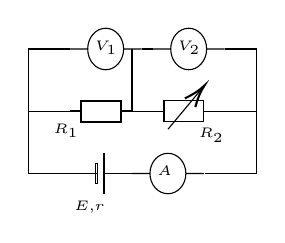
\begin{tikzpicture}[x=0.75pt,y=0.75pt,yscale=-1,xscale=1]
%uncomment if require: \path (0,300); %set diagram left start at 0, and has height of 300

%Straight Lines [id:da14551039289024326] 
\draw    (130,220) -- (150,220) ;
%Straight Lines [id:da3295959610713812] 
\draw    (150,160) -- (130,160) ;
%Shape: Battery [id:dp8317998227732923] 
\draw   (150,220) -- (163.5,220) (166.5,210) -- (166.5,230) (166.5,220) -- (180,220) (162.3,215) -- (163.5,215) -- (163.5,225) -- (162.3,225) -- (162.3,215) -- cycle ;
%Straight Lines [id:da6993800641983081] 
\draw    (130,160) -- (130,220) ;
%Straight Lines [id:da47030402702453067] 
\draw    (215,220) -- (240,220) ;
%Straight Lines [id:da10115275650248856] 
\draw    (240,160) -- (240,220) ;
%Shape: Output [id:dp34471276111404703] 
\draw   (188.65,220) .. controls (188.65,214.62) and (192.52,210.26) .. (197.3,210.26) .. controls (202.08,210.26) and (205.95,214.62) .. (205.95,220) .. controls (205.95,225.38) and (202.08,229.74) .. (197.3,229.74) .. controls (192.52,229.74) and (188.65,225.38) .. (188.65,220) -- cycle (180,220) -- (188.65,220) (214.6,220) -- (205.95,220) ;
%Straight Lines [id:da2535463577123036] 
\draw    (220,190) -- (240,190) ;
%Shape: Resistor [id:dp2889455083490655] 
\draw   (195.4,195) -- (214.6,195) -- (214.6,185) -- (195.4,185) -- (195.4,195) -- cycle (190,190) -- (195.4,190) (214.6,190) -- (220,190) ;
%Straight Lines [id:da6959465546040076] 
\draw    (197.33,198.67) -- (213.71,179.03) ;
\draw [shift={(214.99,177.5)}, rotate = 129.83] [color={rgb, 255:red, 0; green, 0; blue, 0 }  ][line width=0.75]    (10.93,-3.29) .. controls (6.95,-1.4) and (3.31,-0.3) .. (0,0) .. controls (3.31,0.3) and (6.95,1.4) .. (10.93,3.29)   ;
%Straight Lines [id:da7548896744967672] 
\draw    (224.6,160) -- (240,160) ;
%Straight Lines [id:da05255225869571456] 
\draw    (184.6,160) -- (190,160) ;
%Shape: Output [id:dp7402485705608346] 
\draw   (158.65,160) .. controls (158.65,154.48) and (162.52,150) .. (167.3,150) .. controls (172.08,150) and (175.95,154.48) .. (175.95,160) .. controls (175.95,165.52) and (172.08,170) .. (167.3,170) .. controls (162.52,170) and (158.65,165.52) .. (158.65,160) -- cycle (150,160) -- (158.65,160) (184.6,160) -- (175.95,160) ;
%Straight Lines [id:da7775464807313777] 
\draw    (180,190) -- (190,190) ;
%Straight Lines [id:da5256323795807551] 
\draw    (150,190) -- (130,190) ;
%Shape: Resistor [id:dp7893409265728679] 
\draw  [color={rgb, 255:red, 0; green, 0; blue, 0 }  ,draw opacity=1 ][fill={rgb, 255:red, 255; green, 255; blue, 255 }  ,fill opacity=1 ][line width=0.75]  (155.4,185) -- (174.6,185) -- (174.6,195) -- (155.4,195) -- (155.4,185) -- cycle (150,190) -- (155.4,190) (174.6,190) -- (180,190) ;
%Shape: Output [id:dp686244368823177] 
\draw   (198.65,160) .. controls (198.65,154.48) and (202.52,150) .. (207.3,150) .. controls (212.08,150) and (215.95,154.48) .. (215.95,160) .. controls (215.95,165.52) and (212.08,170) .. (207.3,170) .. controls (202.52,170) and (198.65,165.52) .. (198.65,160) -- cycle (190,160) -- (198.65,160) (224.6,160) -- (215.95,160) ;
%Straight Lines [id:da6913018383920955] 
\draw    (180,160) -- (180,190) ;

% Text Node
\draw (191,215) node [anchor=north west][inner sep=0.75pt]  [font=\tiny] [align=left] {$\displaystyle A$};
% Text Node
\draw (161,155) node [anchor=north west][inner sep=0.75pt]  [font=\tiny] [align=left] {$\displaystyle V_{1}$};
% Text Node
\draw (151,232) node [anchor=north west][inner sep=0.75pt]  [font=\tiny] [align=left] {$\displaystyle E$,$\displaystyle r$};
% Text Node
\draw (141,195) node [anchor=north west][inner sep=0.75pt]  [font=\tiny] [align=left] {$\displaystyle R_{1}$};
% Text Node
\draw (201,155) node [anchor=north west][inner sep=0.75pt]  [font=\tiny] [align=left] {$\displaystyle V_{2}$};
% Text Node
\draw (211,197) node [anchor=north west][inner sep=0.75pt]  [font=\tiny] [align=left] {$\displaystyle R_{2}$};
\end{tikzpicture}
\end{center}